\documentclass[11pt]{article}
\usepackage[review]{acl}
% lineno 5.6+ (TeX Live 2026) swaps the margins of the review line numbers in two-column
% mode; put them back on the outer margins. Older lineno versions (Overleaf) are unaffected.
\makeatletter
\@ifpackagelater{lineno}{2026/02/11}{\AtBeginDocument{\switchlinenumbers*}}{}
\makeatother
\usepackage{times}
\usepackage{latexsym}
\usepackage[T1]{fontenc}
\usepackage[utf8]{inputenc}
\usepackage{microtype}
\usepackage{inconsolata}
\usepackage{graphicx}
\usepackage{amsmath}
\usepackage{amssymb}
\usepackage{amsthm}
\usepackage{booktabs}
\usepackage{makecell}
\usepackage{enumitem}
\usepackage{flafter}
\usepackage[table]{xcolor}
\usepackage[most]{tcolorbox}
\usepackage{algorithm}
\usepackage{algpseudocode}
\usepackage{pgfplots}
\pgfplotsset{compat=1.18}

% ---------------------------------------------------------------------
% Theorems and operators (used in Sections 4 and 6)
% ---------------------------------------------------------------------
\newtheorem{proposition}{Proposition}
\DeclareMathOperator*{\argmax}{arg\,max}

% ---------------------------------------------------------------------
% Colours for the front figure and the per-language plot (Sections 5, 8)
% ---------------------------------------------------------------------
\definecolor{pfair}{HTML}{0B3D91}
\definecolor{hybrid}{HTML}{D9622B}
\definecolor{soft}{HTML}{DDE3EC}

% ---------------------------------------------------------------------
% Placeholder and box styles
% ---------------------------------------------------------------------
\definecolor{pframe}{HTML}{3C4A5C}
\definecolor{pback}{HTML}{F7F8FA}
\definecolor{plabel}{HTML}{3C4A5C}
\definecolor{pslot}{HTML}{1F5FA8}

% {placeholder} slots in blue monospace
\newcommand{\ph}[1]{\textcolor{pslot}{\texttt{\{#1\}}}}
% small-caps style section labels
\newcommand{\psec}[1]{\par\medskip{\footnotesize\sffamily\bfseries\color{plabel}#1}\par\smallskip}

\newtcolorbox{pslotbox}[1]{enhanced, colback=white, colframe=gray!30,
  boxrule=0.4pt, arc=2pt, left=6pt, right=6pt, top=4pt, bottom=4pt,
  fontupper=\small, title={#1}, fonttitle=\footnotesize\sffamily\bfseries,
  coltitle=plabel, colbacktitle=gray!10, toptitle=1pt, bottomtitle=1pt}

% Table palette: cool slate blue
\definecolor{headergray}{HTML}{DCE6F2}   % header: soft blue
\definecolor{rowgray}{HTML}{F5F8FC}      % zebra rows: barely-there blue
\definecolor{overallgray}{HTML}{E8EEF7}  % overall row: between the two

% Table palette: sage
% \definecolor{headergray}{HTML}{DDEBE4}
% \definecolor{rowgray}{HTML}{F5FAF7}
% \definecolor{overallgray}{HTML}{E8F2EC}

\title{One Dial from Compression to Parity:\\ A Power-Mean View of Fair BPE Tokenization}

\author{
  Vaibhav Rathore \quad Siddhant Gole \\
  IIT Bombay \\
  \texttt{\{25d1387,26d1384\}@iitb.ac.in}
}

\begin{document}
\maketitle

\begin{abstract}
Subword tokenizers learn their vocabulary from frequency statistics, so languages with
less training text pay more tokens for the same content. Classical BPE minimises the total
token count and ignores this disparity, while Parity-aware BPE equalises the cost across
languages at some loss of compression. Methods between these ends are heuristic and
state no objective. To address this, we show that both ends
are special cases of one objective, a power mean of per-language token costs with exponent
$p$. Its greedy step weights each language's pair counts by its current cost raised to the
power $p-1$, giving classical BPE at $p=1$ and Parity-aware BPE as $p\to\infty$. We call the
tokenizers in between $p$-fair BPE and train them exactly by lazy evaluation, about 20 times
faster than full rescoring. On Hindi, Marathi, Gujarati and English, raising $p$
traces a monotone compression--parity front in all five training samples. At $p=8$, the
Gini coefficient of per-language cost falls by 40\% for a 0.6\% loss in compression. The
% TODO (E3 in experiments.md): this "no language worse off" statement holds for the four-language
% setting only. In the 14-language pilot (reference_results/l14_preview) p-fair raises the cheapest
% languages (Bengali, Hindi) like every fairness rule does; what stays true is that p-fair never
% raises a language that costs MORE than the classical mean, whereas the hybrid does (Gujarati,
% Malayalam). Reword to the under-served form once E3 has error bars (paper_tables.py underserved).
front matches the hybrid baseline, but unlike the hybrid, $p$-fair BPE never raises an
Indian language's cost above its classical cost. Finally, we show that the cost unit and
data balance decide the size and even the direction of the disparity.
\end{abstract}

\section{Introduction}
\label{sec:intro}

% P1: task and why token cost matters
Language models read tokens, not characters, and the cost of a request, its latency and the
amount of text that fits in the context window are all counted in tokens. Byte-pair
encoding (BPE) \citep{gage1994,sennrich2016} builds its vocabulary by repeatedly merging the
most frequent pair of adjacent symbols in a training corpus, so the merges follow the
languages that dominate the corpus, and the same content needs many more tokens in some
languages than in others, up to 15 times more for deployed tokenizers \citep{petrov2023}.
In our setting, a Hindi request to a model with an English-heavy tokenizer costs 21\% more
tokens than its English translation (35.0 vs.\ 29.0 per sentence).

% P2: existing methods sit at two ends, the space between is unprincipled
Existing tokenizers answer this disparity at two opposite ends. Classical BPE minimises the
total number of tokens and accepts whatever disparity results; Parity-aware BPE
\citep{foroutan2026} gives every merge to the language that is currently worst off, which
equalises the cost across languages at some loss of total compression. To reach points in
between, \citet{foroutan2026} propose a hybrid schedule that switches from the classical
rule to the parity rule after a fixed share of merges, and \citet{kanjirangat2026} extend
the parity rule to the $N$ worst-off languages. Both are heuristic interpolations: neither
is derived from an objective that describes the trade-off, so a practitioner cannot state
what the intermediate tokenizers optimise or choose a point on the trade-off deliberately.

% P3: our proposal
We treat vocabulary learning as a multi-objective problem over the vector of per-language
token costs, scalarise it with a weighted power mean of exponent $p$, and show that the
greedy step of this objective is a pair count in which each language is weighted by its
current cost raised to the power $p-1$ (Section~\ref{sec:method}). At $p=1$ the rule is
exactly classical BPE, and as $p\to\infty$ it becomes the rule of Parity-aware BPE; we call
the tokenizers in between \emph{$p$-fair BPE}. We further prove that the score of an
existing pair never increases during training, which allows exact training with a lazy
priority queue \citep{minoux1978} at about 20 times the speed of full rescoring.

% P4: what we find
We evaluate $p$-fair BPE on Hindi, Marathi, Gujarati and English with five samples of
training text and a paired bootstrap on FLORES-200 \citep{nllb2022}, and on 14 languages in
ten scripts at natural data balance with three. Raising $p$ moves the tokenizer monotonically from the classical end to the parity end in
every sample, and at $p=8$ the Gini coefficient of per-language cost falls by 40\% for a
0.6\% loss in compression. The front coincides with that of the hybrid schedule in both settings, where
the two differ by at most 0.003 in Gini at equal compression, so $p$-fair BPE matches the
hybrid and does not dominate it; only at a 128k vocabulary is it fairer than every hybrid
point, by 0.002 to 0.006 in five of five samples. Nevertheless, the two methods distribute
the cost differently: for every $p$ we test, no language that costs more than the classical
mean becomes more expensive, whereas the hybrid raises Marathi with four languages (33.26
vs.\ 32.47 tokens per sentence at 75\% classical merges) and Malayalam and Gujarati with
fourteen. Three further factors decide the outcome more than the merge rule does: a per-byte cost
inverts the parity rule across scripts, sending 99\% of its merges to English; the Gini
coefficient of classical BPE ranges from 0.019 with equal data to 0.051 with eight times as
much English; and intermediate $p$ loses equity as the vocabulary grows from 32k to 256k,
whereas the parity rule does not.

\noindent\textbf{Contributions.} (i) We formulate fair vocabulary learning as the
minimisation of a power mean of per-language token costs and show that its greedy step
contains classical BPE ($p=1$) and Parity-aware BPE ($p\to\infty$) as limits of one rule.
(ii) We prove that pair scores are non-increasing under this rule, which gives an exact
lazy-evaluation trainer about 20 times faster than full rescoring. (iii) We trace the
compression--parity front with error bars on four languages and on 14 languages in ten
scripts, and show that $p$-fair BPE matches the hybrid front in both settings while never
raising the cost of an under-served language above its classical cost. (iv) We show that
the cost unit, the data balance and the vocabulary size decide the size and even the
direction of the disparity, that Worst-$N$ parity and the moving window do not
interpolate, and that a convex vocabulary allocation across scripts is a weaker lever than
the merge rule.

\section{Related Work}
\label{sec:related}

\noindent\textbf{BPE as an optimisation problem.}
BPE was introduced for data compression \citep{gage1994} and adapted to subword
segmentation by \citet{sennrich2016}. \citet{zouhar2023} formalise it as the search for a
merge sequence that maximises the number of tokens saved and bound the approximation ratio
of the greedy algorithm; Unigram tokenization \citep{kudo2018} prunes a large vocabulary
under a likelihood objective. Both objectives are defined on the pooled corpus, with no
notion of cost per language.

\noindent\textbf{Cross-lingual disparity and fair tokenizers.}
\citet{petrov2023} show that the tokenizers of deployed models encode the same content with
very different numbers of tokens across languages, measured on parallel text, the unit we
adopt. Parity-aware BPE \citep{foroutan2026} changes the merge rule: at every step it merges
the most frequent pair of the language with the worst compression on a multi-parallel
development set, and a hybrid schedule and a moving-window variant reach intermediate
tokenizers. \citet{kanjirangat2026} extend the parity rule to the $N$ worst-off languages,
and \citet{lee2026} find that Parity-aware BPE lies on the efficiency--equity frontier for
Southeast Asian languages but becomes less equitable as the vocabulary grows. Other work
changes the input rather than the rule, by rebalancing the data \citep{chung2023unimax} or
by a morphology-driven byte encoding \citep{limisiewicz2024myte}. In all of these, the
intermediate tokenizers come from schedules, a choice of $N$ or data weights, none derived
from an objective over per-language costs.

\noindent\textbf{Vocabulary allocation and Indian languages.}
VoCap \citep{zheng2021vocap} allocates vocabulary per language from its average log
probability, XLM-V \citep{liang2023xlmv} builds per-cluster vocabularies before merging
them, and \citet{brahma2026} set each script cluster's share for 17 Indian languages in
proportion to its share of the union of monolingual vocabularies. SuTRA \citep{rathore2026}
penalises merges that cross morpheme boundaries in Hindi, Marathi and Gujarati, whereas
\citet{arnett2025} find across 70 languages that morphological alignment explains little of
the variance in downstream performance. We use the SuTRA languages as our testbed.

\noindent\textbf{Fairness through scalarisation.}
Power means are a standard scalarisation in multi-objective optimisation
\citep{miettinen1999}; the same family appears as $\alpha$-fair utility in resource
allocation \citep{mo2000fair} and as the Atkinson index in economics \citep{atkinson1970}.
Our trainer builds on the lazy greedy technique of \citet{minoux1978}. To our knowledge,
this family has not been applied to the merge rule of a tokenizer, where it yields a
closed-form weighting of pair counts and an exact lazy trainer.


\section{Problem Formulation}
\label{sec:problem}

\noindent\textbf{Tokenizers and token cost.}
Let $\mathcal{L}$ be a set of $L$ languages. A BPE vocabulary $V$ consists of a base
alphabet and an ordered list of merges, with size bounded by a budget $K$. Each language
$\ell$ has a training text $\mathcal{D}_\ell$ from which merges are learned, and
$c_\ell(a,b)$ denotes the number of occurrences of the adjacent pair $(a,b)$ in
$\mathcal{D}_\ell$ under the current vocabulary. A multi-parallel development set contains
the same $S$ sentences in every language. Let $T_\ell(V)$ be the number of tokens that $V$ produces on the development
sentences of language $\ell$. We define the \emph{token cost} of language $\ell$ as
\begin{equation}
  t_\ell(V) \;=\; \frac{T_\ell(V)}{S},
  \label{eq:cost}
\end{equation}
the average number of tokens needed for one sentence of shared content. A tokenizer is fair
when all $t_\ell$ are close to one another, and efficient when they are small.

\noindent\textbf{Choice of cost unit.}
The denominator in Eq.~\eqref{eq:cost} must not depend on the script: in UTF-8 a Devanagari
character occupies three bytes and a Latin character one, so per byte English appears to be
the most expensive language even when it needs the fewest tokens per sentence, and any rule
that helps the worst-off language then sends its merges to English
(Section~\ref{sec:unitresult}). We therefore measure cost per parallel sentence, following
\citet{petrov2023} and \citet{foroutan2026}.

\noindent\textbf{A multi-objective view.}
The costs $\mathbf{t}(V)=(t_1(V),\dots,t_L(V))$ form a vector of objectives to be made small
together:
\begin{equation}
  \min_{|V|\le K}\; \mathbf{t}(V).
  \label{eq:mo}
\end{equation}
A vocabulary is Pareto-optimal for Eq.~\eqref{eq:mo} if no other vocabulary of size at most
$K$ lowers the cost of one language without raising that of another, and the cost vectors
of Pareto-optimal vocabularies form the compression--parity front. Existing tokenizers each
commit to one point on it: classical BPE favours total compression, Parity-aware BPE the
worst-off language.

\noindent\textbf{Power-mean scalarisation.}
To trace the front with a single parameter, we scalarise Eq.~\eqref{eq:mo} with a weighted
power mean,
\begin{equation}
  \min_{|V|\le K}\; F_p(V) \;=\;
  \Bigl(\sum_{\ell\in\mathcal{L}} \pi_\ell\, t_\ell(V)^{p}\Bigr)^{1/p},
  \qquad p\in[1,\infty],
  \label{eq:obj}
\end{equation}
with weights $\pi_\ell>0$ that sum to one. We set $\pi_\ell$ to the share of language $\ell$
in the training text, measured in development-sentence units, for the reason given in
Section~\ref{sec:rule}. The exponent $p$ sets how strongly expensive
languages are emphasised: at $p=1$, $F_1=\sum_\ell \pi_\ell t_\ell$ is the weighted average
cost that classical BPE reduces; as $p\to\infty$, $F_p\to\max_\ell t_\ell$, the cost of the
worst-off language that Parity-aware BPE reduces; for $1<p<\infty$, $F_p$ lies between the
two and gives more weight to a language the more expensive it is. For finite $p$ and positive weights, $F_p$ is strictly increasing in every $t_\ell$.
Consequently, an exact minimiser of Eq.~\eqref{eq:obj} is Pareto-optimal for
Eq.~\eqref{eq:mo}, while a minimiser of the max at $p=\infty$ is only guaranteed to be
weakly Pareto-optimal. In practice, we minimise Eq.~\eqref{eq:obj} greedily, one merge at a
time (Section~\ref{sec:method}), so the curve we measure is the front of the greedy
algorithm rather than the exact Pareto front.

\noindent\textbf{Evaluation measures.}
For parity, we report the Gini coefficient of the per-language costs on a held-out parallel
test set,
\begin{equation}
  G \;=\; \frac{\sum_{i,j\in\mathcal{L}} |t_i - t_j|}{2L^2\,\bar t},
  \label{eq:gini}
\end{equation}
where $\bar t$ is the mean cost ($G=0$ when every language costs the same). For efficiency,
we report compression in bytes per token on the training text, the quantity classical BPE
greedily maximises, and additionally on the balanced test set.

\section{Method: $p$-fair BPE}
\label{sec:method}

Like classical BPE, $p$-fair BPE builds the vocabulary one merge at a time and chooses each
merge greedily: we derive the merge rule implied by Eq.~\eqref{eq:obj}, show that it contains
classical and Parity-aware BPE as limits, and give an exact and fast training algorithm.

\subsection{The greedy merge rule}
\label{sec:rule}

Merging a pair $(a,b)$ replaces each of its occurrences by one symbol, so the token count
of a text falls by the number of occurrences of the pair. The pair counts $c_\ell$ come from
the training text, whereas the costs $t_\ell$ are measured on the development set. To
connect the two, we assume that a pair occurs in the development text of language $\ell$ at
the same rate as in its training text. Let $N_\ell$ denote the size of $\mathcal{D}_\ell$
expressed in development sentences, that is, its length divided by the average length of a
development sentence in language $\ell$. Under this assumption, merging $(a,b)$ lowers
$T_\ell$ by $S\,c_\ell(a,b)/N_\ell$ and therefore lowers $t_\ell$ by $c_\ell(a,b)/N_\ell$.

\begin{proposition}
\label{prop:rule}
Let $\pi_\ell = N_\ell/\sum_k N_k$. To first order, the merge that decreases $F_p$ the most
is
\begin{equation}
  (a,b)^\star \;=\; \argmax_{(a,b)}\; s_p(a,b), \qquad
  s_p(a,b) = \sum_{\ell\in\mathcal{L}} t_\ell^{\,p-1}\, c_\ell(a,b).
  \label{eq:rule}
\end{equation}
\end{proposition}
The proof, a first-order expansion of $F_p$, is in Appendix~\ref{app:proofs}.


Thus, the rule is a pair count in which each language is weighted by its current cost raised
to the power $p-1$. The weights change after every merge; we update every $t_\ell$ exactly
by applying the merge to the development set, so only the per-merge choice relies on the
first-order approximation.

With Hindi at 35.0 tokens per sentence and English at 29.0, as under classical BPE in our
experiments, a Hindi pair counts $(35.0/29.0)^{p-1}$ times as much as an English pair of the
same frequency: 1.2 times at $p=2$ and 3.7 times at $p=8$.

\subsection{Classical and Parity-aware BPE as limits}
\label{sec:limits}

The rule in Eq.~\eqref{eq:rule} has two limits. At $p=1$ every weight equals one,
$s_1(a,b)=\sum_\ell c_\ell(a,b)$ is the count of the pair in the pooled training text, and
the rule is exactly classical BPE. As $p\to\infty$, dividing $s_p$ by
$(\max_\ell t_\ell)^{p-1}$ does not change the $\argmax$; the weight of the worst-off
language is then one and every other weight tends to zero, so the rule selects the most
frequent pair of the worst-off language. This is the base rule of Parity-aware BPE
\citep{foroutan2026} with cost measured per parallel sentence, and corresponds to a
subgradient step on $\max_\ell t_\ell$. For $1<p<\infty$ every language keeps a positive weight: unlike the parity rule (one language
per merge) and the Worst-$N$ rule \citep{kanjirangat2026} (the $N$ worst-off weighted
equally), $p$-fair BPE weights all languages continuously by their cost, and unlike the
hybrid schedule \citep{foroutan2026} it uses one parameter that is constant throughout
training.

\subsection{Exact training by lazy evaluation}
\label{sec:lazy}

Efficient implementations of classical BPE keep the pair counts in a priority queue and
update only the pairs that a merge touches. In Eq.~\eqref{eq:rule} the weights change after
every merge, so every score changes, and rescoring all $|\mathcal{P}|$ pairs at each of the
$\sim$31{,}000 steps costs $O(|\mathcal{P}|\,L)$ per step. The following property avoids this.

\begin{proposition}
\label{prop:lazy}
For $p\ge1$, the score $s_p(a,b)$ of a pair that already exists never increases during
training.
\end{proposition}
The proof is in Appendix~\ref{app:proofs}.


Consequently, a stored score is always an upper bound on the current score. We keep the
pairs in a max-heap keyed by their stored scores, pop the top entry and recompute its score
with the current weights: if it is unchanged, the entry is the exact maximiser of
Eq.~\eqref{eq:rule}, since every other stored score bounds its current score from above;
otherwise we push it back with the new score and repeat (Algorithm~\ref{alg:pfair} in
Appendix~\ref{app:impl}). This is the lazy greedy technique of \citet{minoux1978}, and it
returns the same merge as full rescoring at every step. For $p=\infty$ we keep one heap per
language keyed by $c_\ell$ and pop from the heap of the worst-off language.


\section{Experiments}
\label{sec:results}

\subsection{Experimental setup}
\label{sec:setup}

\noindent\textbf{Languages and data.}
We used Hindi, Marathi and Gujarati, the SuTRA languages \citep{rathore2026}, together with
English as the dominant language. Training text comes from the verified split of Sangraha
\citep{khan2024}, with about 20 million characters for each Indian language and 80 million
for English (preprocessing in Appendix~\ref{app:impl}). Parallel text comes from FLORES-200
\citep{nllb2022}: the \emph{dev} split (997 sentences) measures the costs $t_\ell$ during
training, and the \emph{devtest} split (1012 sentences) gives every reported number.

\noindent\textbf{Tokenizers.}
All tokenizers are character-level BPE with whitespace pre-tokenization, a word-start marker
and a vocabulary of 32{,}000 (alphabet: every character with at least five occurrences,
about 1000; rarer characters map to an unknown token). We trained $p\in\{1,2,4,8,16,32,\infty\}$, where $p=1$ is classical BPE and
$p=\infty$ is our implementation of the base rule of Parity-aware BPE. As the main baseline,
we used the \textbf{hybrid} schedule of \citet{foroutan2026}, which learns the first 50\%,
75\% or 90\% of the merges with the classical rule and the rest with the parity rule. We
also trained the Worst-$N$ rule of \citet{kanjirangat2026} with $N\in\{2,3\}$ and the
moving-window variant of \citet{foroutan2026} with a window of 100 merges and $\alpha=2$.
All baselines are our own character-level implementations of the published rules, whose
originals are byte-level.

\noindent\textbf{Protocol.}
Every configuration was trained on five non-overlapping samples of Sangraha (mean and
standard deviation reported), and the devtest sentences were resampled 1000 times with
replacement (a paired bootstrap) to separate test-set variance from training-data variance.

\noindent\textbf{Implementation and checks.}
The trainer is written in Rust. The lazy trainer produces merge lists identical to full
rescoring for every rule in this paper, the $p=1$ setting reproduces an independent textbook
BPE merge for merge, and the evaluator's token counts equal the trainer's own totals.
Training times are given in Appendix~\ref{app:impl}.

\subsection{Raising $p$ traces the compression--parity front}

Under classical BPE, a Hindi sentence costs 35.0 tokens and its English translation 29.0, a
difference of 21\% (Table~\ref{tab:perlang}, Appendix~\ref{app:perlang}); the cause is
visible in Table~\ref{tab:front}, where English, with four sevenths of the training text,
leads 49\% of the merges. As $p$ grows, Hindi and Gujarati become cheaper, English becomes more expensive, and at
$p=\infty$ the four costs meet near 32 tokens (Table~\ref{tab:perlang}). In the two summary
measures (Table~\ref{tab:front}, Fig.~\ref{fig:front}), the Gini coefficient falls at every
step, from 0.038 to 0.003, and so does compression of the training text, from 6.91 to 6.63
bytes per token.

The price of parity is uneven along the front: at $p=8$ the Gini coefficient is 40\% lower
than under classical BPE for 0.6\% less compression, at $p=16$ 60\% lower for 1.3\%, and full
parity costs 4.0\%, so a large part of the disparity can be removed for a small part of the
cost of removing all of it. On devtest, where every language has
the same content, intermediate values of $p$ even compress better than classical BPE (8.89
vs.\ 8.72 bytes per token at $p=16$): classical BPE optimises compression of the mostly
English training mixture, whereas a balanced test set rewards the vocabulary that $p$-fair
BPE moves to the other languages, so whether the loss in Fig.~\ref{fig:front} is a real cost
depends on the mixture the tokenizer meets in deployment.

\begin{table*}[t]
\centering
\small
\begin{tabular}{lccccc}
\toprule
 & Gini of cost & \multicolumn{2}{c}{Compression (bytes/token)} & Merges led & Gini diff.\ at\\
\cmidrule(lr){3-4}
Tokenizer & (devtest) $\downarrow$ & training text $\uparrow$ & devtest $\uparrow$ & by English & matched compr.\\
\midrule
Classical ($p=1$) & $0.0380\pm0.0002$ & $6.910\pm0.004$ & $8.719\pm0.007$ & 49\% & --\\
$p=2$  & $0.0347\pm0.0002$ & $6.907\pm0.004$ & $8.761\pm0.006$ & 47\% & --\\
$p=4$  & $0.0298\pm0.0002$ & $6.897\pm0.004$ & $8.818\pm0.004$ & 43\% & --\\
$p=8$  & $0.0229\pm0.0002$ & $6.868\pm0.004$ & $8.868\pm0.005$ & 38\% & --\\
$p=16$ & $0.0152\pm0.0002$ & $6.818\pm0.005$ & $8.889\pm0.007$ & 34\% & --\\
$p=32$ & $0.0084\pm0.0001$ & $6.760\pm0.006$ & $8.882\pm0.004$ & 30\% & --\\
Parity-aware ($p=\infty$) & $0.0028\pm0.0004$ & $6.634\pm0.007$ & $8.830\pm0.006$ & 23\% & --\\
\midrule
Hybrid, 90\% classical & $0.0270\pm0.0002$ & $6.891\pm0.003$ & $8.788\pm0.005$ & 44\% & $-0.0014\pm0.0004$ (0/5)\\
Hybrid, 75\% classical & $0.0180\pm0.0005$ & $6.827\pm0.004$ & $8.821\pm0.008$ & 37\% & $+0.0013\pm0.0003$ (5/5)\\
Hybrid, 50\% classical & $0.0023\pm0.0004$ & $6.651\pm0.004$ & $8.834\pm0.005$ & 25\% & $-0.0012\pm0.0005$ (0/5)\\
\bottomrule
\end{tabular}
\caption{Parity and compression at 32k with English at four times the text of each other
language; mean $\pm$ standard deviation over five samples. ``Merges led by English'': share
of merges to whose score English contributes most. ``Gini diff.'': hybrid Gini minus the
$p$-fair front interpolated at the same training-text compression (positive: $p$-fair
fairer), with the number of samples in which $p$-fair is fairer.}
\label{tab:front}
\end{table*}

\begin{figure}[t]
\centering
\resizebox{\columnwidth}{!}{%
\begin{tikzpicture}
\begin{axis}[
  width=9cm, height=4.6cm,
  xlabel={compression of training text (bytes per token) $\rightarrow$ better},
  ylabel={Gini of per-language cost (lower is fairer)},
  xmin=6.56, xmax=6.97, ymin=-0.003, ymax=0.043,
  xtick={6.6,6.7,6.8,6.9}, ytick={0,0.01,0.02,0.03,0.04},
  scaled y ticks=false,
  yticklabel style={/pgf/number format/fixed,/pgf/number format/precision=2},
  grid=major, grid style={draw=soft},
  legend style={font=\small, at={(0.97,0.05)}, anchor=south east, draw=none, fill=white},
  legend cell align=left,
  tick label style={font=\small}, label style={font=\small}]
\addplot[mark=*, mark size=2pt, thick, color=pfair,
  error bars/.cd, x dir=both, x explicit, y dir=both, y explicit]
  table[col sep=comma, x=cr, y=gini, x error=cr_err, y error=gini_err]{data/paper_chart_pfair.csv};
\addplot[only marks, mark=square*, mark size=2.2pt, color=hybrid,
  error bars/.cd, x dir=both, x explicit, y dir=both, y explicit]
  table[col sep=comma, x=cr, y=gini, x error=cr_err, y error=gini_err]{data/paper_chart_hybrid.csv};
\addplot[only marks, mark=triangle*, mark size=2.8pt, color=black!65,
  error bars/.cd, x dir=both, x explicit, y dir=both, y explicit]
  table[col sep=comma, x=cr, y=gini, x error=cr_err, y error=gini_err]{data/paper_chart_other.csv};
\legend{$p$-fair BPE, hybrid baseline, Worst-$N$ / window}
\node[font=\footnotesize, text=pfair, anchor=east] at (axis cs:6.9030,0.0390) {classical ($p=1$)};
\node[font=\footnotesize, text=pfair, anchor=east] at (axis cs:6.8900,0.0303) {$p=4$};
\node[font=\footnotesize, text=pfair, anchor=east] at (axis cs:6.8610,0.0235) {$p=8$};
\node[font=\footnotesize, text=pfair, anchor=east] at (axis cs:6.8100,0.0159) {$p=16$};
\node[font=\footnotesize, text=pfair, anchor=east] at (axis cs:6.7530,0.0092) {$p=32$};
\node[font=\footnotesize, text=pfair, anchor=south west] at (axis cs:6.5680,0.0048) {Parity-aware ($p=\infty$)};
\node[font=\footnotesize, text=hybrid, anchor=north west] at (axis cs:6.8950,0.0262) {90\%};
\node[font=\footnotesize, text=hybrid, anchor=north west] at (axis cs:6.8310,0.0172) {75\%};
\node[font=\footnotesize, text=hybrid, anchor=north west] at (axis cs:6.6560,0.0016) {50\%};
\end{axis}
\end{tikzpicture}}
\caption{The compression--parity front: means of five samples, bars one standard deviation
(mostly smaller than the marker). The hybrid (share of classical merges) lies on the curve;
Worst-$N$ ($N=2,3$) and the moving window (triangles) coincide with the parity end.}
\label{fig:front}
\end{figure}

The front is reliable. Every increase in $p$ lowers both the Gini coefficient and the
compression of the training text in five of five samples, and the standard deviation of the
Gini coefficient across samples (0.0001 to 0.0005) is 10 to 30 times smaller than the
difference between neighbouring values of $p$. Resampling the test sentences leads to the
same conclusion: the 95\% interval for classical BPE is $[0.036,0.040]$ and for $p=8$ it is
$[0.021,0.025]$, and each step up in $p$ lowers the Gini coefficient in at least 99.7\% of
the 1000 resamples.

\subsection{Comparison with the hybrid, Worst-$N$ and moving-window baselines}
\label{sec:hybrid}

The hybrid points in Fig.~\ref{fig:front} lie on the $p$-fair front. To compare the two
methods at equal compression, we interpolated the $p$-fair front at the compression of each
hybrid tokenizer, separately in each sample, and took the difference in Gini (last column
of Table~\ref{tab:front}). The differences are about 0.001, consistent in sign across the
five samples, and go in both directions: $p$-fair BPE is slightly fairer at 75\%, the hybrid
at 50\% and 90\%, so neither method dominates the other. The hybrid with 50\% classical merges is at least as good as pure Parity-aware BPE on both
measures, in line with its motivation in \citet{foroutan2026}.


Worst-$N$ parity and the moving window do not interpolate in this setting
(Table~\ref{tab:worstn}, Appendix~\ref{app:perlang}). With $N=2$ or $N=3$ the Worst-$N$ rule
pools the Indian languages, whose classical costs lie within 8\% of one another, so it
behaves like the parity rule and lands at the parity end of the front (Gini 0.0025 to
0.0029 against 0.0028 for Parity-aware BPE), as does the moving window; their Gini at
matched compression differs from the $p$-fair front by 0.0002 to 0.0006, within the
sample-to-sample spread. Section~\ref{sec:multi} tests these rules where several languages
are under-served at different levels.

Nevertheless, the hybrid and $p$-fair BPE distribute the cost differently (Table~\ref{tab:perlang}).
For every value of $p$ we test, no Indian language costs more than under classical BPE in
this setting. In contrast, the parity phase of the hybrid equalises the three Indian languages with one
another, which raises Marathi above its classical cost at 90\% and 75\% classical merges,
by up to 0.8 tokens per sentence (33.26 vs.\ 32.47 at 75\%). At similar compression, $p$-fair BPE
with $p=8$ keeps Marathi at 31.90 while leaving a wider spread between the Indian languages.
The general form of this property, which also holds with 14 languages, where every rule
raises the cheapest ones (Section~\ref{sec:multi}), is that $p$-fair BPE never raises a
language that costs more than the classical mean, whereas the hybrid does. Consequently,
the choice between the two depends on the goal: the hybrid moves closer to equal cost among
the Indian languages, whereas $p$-fair BPE makes none of the under-served ones worse off
than classical BPE.



\section{Ablations and Analysis}
\label{sec:ablation}

% Rows and cells marked "--" are planned experiments without results yet.
% Replace them, and rewrite the matching "Planned" paragraphs, once runs finish.

\subsection{The cost unit decides the outcome}
\label{sec:unitresult}

To test the choice of cost unit (Section~\ref{sec:problem}), we train the parity rule with
cost measured per byte instead of per parallel sentence (Table~\ref{tab:byte}). Per byte,
English becomes the worst-off language, and the parity rule gives it 99\% of the merges.
Measured by what a user pays, the result is the opposite of the intention: the Indian
languages need about twice as many tokens per sentence as under classical BPE (63.6 vs.\
35.0 for Hindi), while English needs fewer (26.6 vs.\ 29.0). Thus, a per-byte cost inverts
the parity rule across scripts, and the cost must be measured on shared content.

\begin{table}[t]
\centering
\small
\resizebox{\columnwidth}{!}{%
\begin{tabular}{lcccc}
\toprule
Tokenizer & Hindi & Marathi & Gujarati & English\\
\midrule
Classical BPE & 35.0 & 32.5 & 34.4 & 29.0\\
Parity-aware, cost per byte & 63.6 & 70.6 & 66.5 & 26.6\\
Parity-aware, cost per sentence & 32.1 & 32.5 & 32.3 & 32.5\\
\bottomrule
\end{tabular}}
\caption{Tokens per sentence on devtest when the training cost is measured per byte
(single run) or per parallel sentence (five-sample mean, Table~\ref{tab:perlang}).}
\label{tab:byte}
\end{table}

\subsection{Data balance and vocabulary size}
\label{sec:sens}

To measure how much the disparity depends on the setting, we repeat the experiment with
other amounts of English and with larger vocabularies (Table~\ref{tab:sens}). The direction
is the same in every setting: the Gini coefficient and the compression fall at every step
in $p$. However, the size of the problem changes considerably with data balance. With equal
amounts of text, classical BPE is already close to parity (Gini 0.019), and full parity costs
1.1\% of compression. With eight times as much English, the Gini coefficient is 0.051, a
Hindi sentence costs 30\% more tokens than its English translation, and full parity costs
7.0\%. Moreover, with equal data the remaining disparity is not between English and the
Indian languages, since English (31.7 tokens) lies between Marathi (30.4) and Hindi (33.3).

Doubling the vocabulary to 64k leaves the Gini coefficient of both classical BPE (0.038) and
Parity-aware BPE (0.003) unchanged. Thus, between 32k and 64k we do not observe the loss of
equity that \citet{lee2026} report for Parity-aware BPE at larger vocabularies.

\noindent\textbf{Planned: 128k vocabulary.}
Since Parity-aware BPE bounds only the worst-off language, \citet{lee2026} find that the
dominant language keeps acquiring merges as the vocabulary grows. For finite $p$, every
language keeps a positive weight in Eq.~\eqref{eq:rule}, so we expect intermediate $p$ to
be less affected. At 128k, the Gini coefficient is -- for classical BPE, -- for $p=8$ and --
for Parity-aware BPE.

\begin{table*}[t]
\centering
\small
\begin{tabular}{llcccccc}
\toprule
English & Vocab. & $p=1$ & $p=2$ & $p=4$ & $p=8$ & $p=\infty$ & Cost of parity\\
\midrule
$1\times$ & 32k & 0.0186 & 0.0172 & 0.0148 & 0.0117 & 0.0034 & 1.1\%\\
$4\times$ $\dagger$ & 32k & 0.0380 & 0.0347 & 0.0298 & 0.0229 & 0.0028 & 4.0\%\\
$8\times$ & 32k & 0.0505 & 0.0461 & 0.0383 & 0.0298 & 0.0033 & 7.0\%\\
$4\times$ & 64k & 0.0378 & 0.0353 & 0.0313 & 0.0255 & 0.0032 & 5.1\%\\
$4\times$ & 128k & -- & -- & -- & -- & -- & --\\
\bottomrule
\end{tabular}
\caption{Gini coefficient of per-language cost in other settings, and the compression lost
by going from classical to Parity-aware BPE. The row marked $\dagger$ is the five-sample mean
of Table~\ref{tab:front}; the others are single runs.}
\label{tab:sens}
\end{table*}

\subsection{Comparison with Worst-$N$ parity and the moving window (planned)}
\label{sec:worstn}

The Worst-$N$ rule \citep{kanjirangat2026} offers a second way to interpolate, by pooling
the training counts of the languages whose cost is at least the mean cost of the $N$
worst-off ones. The moving-window variant of \citet{foroutan2026} instead forbids a
language that led more than $\alpha W/L$ of the last $W$ merges ($W=100$, $\alpha=2$). We
train both in the same setting (Table~\ref{tab:worstn}); $N=1$ coincides with the parity
rule up to ties. At matched compression, the Gini difference between Worst-$N$ and $p$-fair
BPE is --, and between the moving window and $p$-fair BPE is --.

\begin{table}[t]
\centering
\small
\begin{tabular}{lcc}
\toprule
Tokenizer & Gini $\downarrow$ & Compression $\uparrow$\\
\midrule
Worst-$N$, $N=1$ ($=p{=}\infty$) & 0.0028 & 6.634\\
Worst-$N$, $N=2$ & -- & --\\
Worst-$N$, $N=3$ & -- & --\\
Moving window ($W=100$, $\alpha=2$) & -- & --\\
$p$-fair, $p=8$ & 0.0229 & 6.868\\
$p$-fair, $p=32$ & 0.0084 & 6.760\\
\bottomrule
\end{tabular}
\caption{Worst-$N$ parity against $p$-fair BPE at 32k with English at $4\times$.
Compression is bytes per token on the training text.}
\label{tab:worstn}
\end{table}

\subsection{Morphology penalty (planned)}
\label{sec:morph}

To add morphological alignment as a third axis, we subtract a penalty for merges that join
symbols from different morphemes:
\begin{equation}
  (a,b)^\star = \argmax_{(a,b)}\; s_p(a,b) - \lambda\,\beta(a,b),
  \label{eq:morph}
\end{equation}
where $\beta(a,b)=\sum_\ell t_\ell^{\,p-1}\beta_\ell(a,b)$ and $\beta_\ell(a,b)$ counts the
occurrences of the pair in language $\ell$ whose junction is a morpheme boundary according
to the SuTRA segmentations \citep{rathore2026}; an occurrence that crosses a boundary thus
contributes $(1-\lambda)$ of its weight instead of 1. For $0\le\lambda\le1$ every term of
the score stays non-negative and non-increasing, so Proposition~\ref{prop:lazy} and the
lazy trainer remain exact; $\lambda=1$ ignores crossing occurrences entirely. Boundaries are
known only for words in the segmentation lexicon, and the lexicon is disjoint from the
held-out words on which boundary F1 is measured. Table~\ref{tab:morph} reports boundary F1
against the held-out SuTRA gold segmentations. Increasing $\lambda$ changes boundary F1 by
--, at a cost of -- in Gini and -- in compression.

\begin{table}[t]
\centering
\small
\resizebox{\columnwidth}{!}{%
\begin{tabular}{llccccc}
\toprule
 & & & & \multicolumn{3}{c}{Boundary F1 $\uparrow$}\\
\cmidrule(lr){5-7}
$p$ & $\lambda$ & Gini $\downarrow$ & Compr. $\uparrow$ & hi & mr & gu\\
\midrule
1 & 0 & 0.0380 & 6.910 & -- & -- & --\\
1 & 0.5 & -- & -- & -- & -- & --\\
1 & 1 & -- & -- & -- & -- & --\\
8 & 0 & 0.0229 & 6.868 & -- & -- & --\\
8 & 0.5 & -- & -- & -- & -- & --\\
8 & 1 & -- & -- & -- & -- & --\\
$\infty$ & 0 & 0.0028 & 6.634 & -- & -- & --\\
$\infty$ & 0.5 & -- & -- & -- & -- & --\\
$\infty$ & 1 & -- & -- & -- & -- & --\\
\bottomrule
\end{tabular}}
\caption{Effect of the morphology penalty. Compression is bytes per token on the training
text; boundary F1 is measured against the SuTRA gold segmentations.}
\label{tab:morph}
\end{table}

\subsection{Vocabulary allocation across scripts (planned)}
\label{sec:alloc}

A complementary question is how a fixed vocabulary of size $K$ should be divided between
scripts (Devanagari, Gujarati and Latin). We fit a cost curve $t_c(k)=a_c k^{-b_c}+d_c$ per
script $c$ and solve $\min_k \sum_c \pi_c\, t_c(k_c)^p$ subject to $\sum_c k_c=K$, which is
convex for $p\ge1$ and is solved by water-filling (Appendix~\ref{app:alloc}). We compare it
with a uniform split, a split proportional to the data share of each script, and the
union-proportion rule of \citet{brahma2026}, and we report a joint tokenizer of the same
size without any allocation as a reference (Table~\ref{tab:alloc}).

\begin{table}[t]
\centering
\small
\begin{tabular}{lcc}
\toprule
Allocation & Gini $\downarrow$ & Compression $\uparrow$\\
\midrule
Joint, $p=1$ (no allocation) & 0.0380 & 6.910\\
Joint, $p=8$ (no allocation) & 0.0229 & 6.868\\
Uniform split & -- & --\\
Data-proportional split & -- & --\\
Union proportion \citep{brahma2026} & -- & --\\
Convex, $p=1$ & -- & --\\
Convex, $p=8$ & -- & --\\
\bottomrule
\end{tabular}
\caption{Vocabulary allocation across scripts at a total budget of 32k.}
\label{tab:alloc}
\end{table}

\subsection{Scaling to 14 languages and natural data balance (planned)}
\label{sec:multi}

With four languages and one dominant language, the front is one-dimensional and a single
switch point suffices to trace it, which may explain why the hybrid schedule matches
$p$-fair BPE. To test the rule where several languages are under-served at different
levels, we train on 14 languages in 10 scripts (Hindi, Marathi, Gujarati, Bengali, Punjabi,
Odia, Assamese, Sanskrit, Tamil, Telugu, Kannada, Malayalam, Urdu and English) with the
amount of text of each language proportional to the size of its Sangraha split, so that the
largest language has about 40 times the text of the smallest, at a 64k vocabulary
(Table~\ref{tab:multi}). At matched compression, $p$-fair BPE is -- than the hybrid by --
in Gini, -- than Worst-$N$ by --, and the largest increase of any language's cost over its
classical cost is -- for $p$-fair BPE and -- for the hybrid.

\begin{table*}[t]
\centering
\small
\begin{tabular}{lcccc}
\toprule
Tokenizer & Gini $\downarrow$ & Max/min $\downarrow$ & Compression $\uparrow$ & Worst regression vs.\ classical $\downarrow$\\
\midrule
Classical ($p=1$) & -- & -- & -- & 1.000\\
$p=4$ & -- & -- & -- & --\\
$p=8$ & -- & -- & -- & --\\
$p=16$ & -- & -- & -- & --\\
Parity-aware ($p=\infty$) & -- & -- & -- & --\\
Hybrid, 75\% classical & -- & -- & -- & --\\
Worst-$N$, $N=3$ & -- & -- & -- & --\\
Moving window & -- & -- & -- & --\\
\bottomrule
\end{tabular}
\caption{Fourteen languages at natural data balance, 64k vocabulary. ``Worst regression''
is $\max_\ell t_\ell/t_\ell^{\mathrm{classical}}$ over the non-English languages.}
\label{tab:multi}
\end{table*}

\subsection{Language-model evaluation (planned)}
\label{sec:downstream}

Token cost is what a user pays, but a fairer tokenizer could in principle make the model
worse at the languages it helps. To test this, we train one small language model per
tokenizer on the same training text (Appendix~\ref{app:impl}) and report bits per byte on
FLORES devtest, a measure that does not depend on the tokenization
(Table~\ref{tab:downstream}). Across tokenizers, the mean bits per byte differs by at most
--, and the spread between languages changes from -- under classical BPE to -- at $p=8$.
Optionally, we also report the number of tokens per technical term on CSTT term lists.

\begin{table}[t]
\centering
\small
\resizebox{\columnwidth}{!}{%
\begin{tabular}{lccccc}
\toprule
Tokenizer & hi & mr & gu & en & Mean\\
\midrule
Classical ($p=1$) & -- & -- & -- & -- & --\\
$p$-fair, $p=8$ & -- & -- & -- & -- & --\\
$p$-fair, $p=32$ & -- & -- & -- & -- & --\\
Hybrid, 75\% classical & -- & -- & -- & -- & --\\
Parity-aware ($p=\infty$) & -- & -- & -- & -- & --\\
\bottomrule
\end{tabular}}
\caption{Bits per byte of a 6-layer language model on FLORES-200 devtest (lower is better),
one model per tokenizer, same training text.}
\label{tab:downstream}
\end{table}

\section{Conclusion}
\label{sec:conclusion}

We address the trade-off between compression and cross-lingual parity in subword
tokenization by treating the per-language token costs as a vector of objectives. Its
power-mean scalarisation yields a greedy merge rule that weights each language's pair counts
by its current cost raised to the power $p-1$, which contains classical BPE at $p=1$ and
Parity-aware BPE as $p\to\infty$. Since pair scores never increase under this rule, the
resulting $p$-fair BPE trains exactly by lazy evaluation, about 20 times faster than full
rescoring. On Hindi, Marathi, Gujarati and English, raising $p$ traces a monotone and
repeatable front, on which a 40\% reduction in the Gini coefficient costs 0.6\% of
compression. The front coincides with that of the hybrid schedule, so the contribution is a
principled formulation of the existing trade-off rather than a tokenizer that dominates it.
Nevertheless, the formulation exposes a difference in how cost is distributed, since
% TODO (E3 in experiments.md): this "no language worse off" statement holds for the four-language
% setting only. In the 14-language pilot (reference_results/l14_preview) p-fair raises the cheapest
% languages (Bengali, Hindi) like every fairness rule does; what stays true is that p-fair never
% raises a language that costs MORE than the classical mean, whereas the hybrid does (Gujarati,
% Malayalam). Reword to the under-served form once E3 has error bars (paper_tables.py underserved).
$p$-fair BPE makes no Indian language more expensive than under classical BPE. Moreover, our
analysis shows that the cost unit and the training data balance decide the size, and even
the direction, of the disparity more than the merge rule does.

\noindent\textbf{Practical takeaways.} First, measure the cost on parallel content and not
per byte, since a per-byte cost inverts the parity rule across scripts. Second, report the
data balance alongside any parity result, since the same method removes 1.1\% or 7.0\% of
compression depending on how much English is present. Third, choose $p$ by the acceptable
loss in compression, since most of the disparity is removed well before full parity.

\noindent\textbf{Open directions.} The formulation extends naturally to further axes and
settings: a morphology penalty within the same rule (Section~\ref{sec:morph}), a convex
allocation of the vocabulary across scripts (Section~\ref{sec:alloc}), large vocabularies
where Parity-aware BPE loses equity \citep{lee2026}, and a $p$-fair variant of Unigram
pruning \citep{kudo2018}.

\section*{Limitations}

\noindent\textbf{Scale and languages.} We train on 140 million characters and evaluate on
1012 parallel sentences in four languages, three of which are closely related. The
sensitivity runs in Table~\ref{tab:sens} are single runs. Results may differ for larger
corpora, more languages or more distant scripts.

\noindent\textbf{Data balance as a design choice.} The size of the disparity depends mainly
on how much English is in the training text, and our main setting with four times as much
English is an assumption. Our conclusions should be read together with
Table~\ref{tab:sens}.

\noindent\textbf{Greedy, first-order steps.} Proposition~\ref{prop:rule} is a first-order
argument, and it assumes that pair frequencies in the development set match those in the
training text. Greedy merging carries no optimality guarantee for $p>1$, so the measured
curve is the front of the greedy algorithm and not the Pareto front of Eq.~\eqref{eq:obj}.

\noindent\textbf{Re-implemented baselines.} Parity-aware BPE, the hybrid schedule, the
moving window and Worst-$N$ are our own character-level implementations of the published
rules, whereas the originals are byte-level.

\noindent\textbf{Intrinsic evaluation.} We measure token cost and compression only. Lower
token cost does not by itself guarantee better downstream performance, and a model-level
evaluation is required to confirm that the gains matter in use.

\bibliography{main}

\clearpage
\appendix
% Appendix. Sections marked "(planned)" and cells marked "--" are filled from
% the experiments in experiments.md (repository root).

\section{Per-language costs along the front}
\label{app:perlang}

\begin{figure}[h]
\centering
\resizebox{\columnwidth}{!}{%
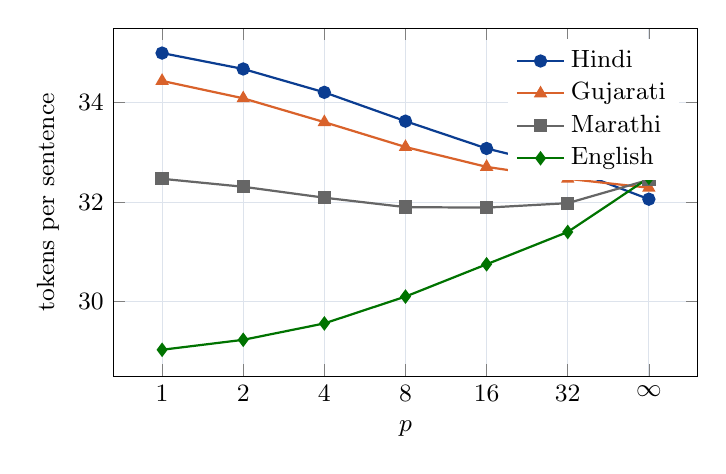
\begin{tikzpicture}
\begin{axis}[
  width=9cm, height=6cm,
  xlabel={$p$}, ylabel={tokens per sentence},
  symbolic x coords={1,2,4,8,16,32,$\infty$}, xtick=data,
  ymin=28.5, ymax=35.5,
  grid=major, grid style={draw=soft},
  legend style={font=\small, at={(0.97,0.97)}, anchor=north east, draw=none, fill=white},
  legend cell align=left,
  tick label style={font=\small}, label style={font=\small}]
\addplot[mark=*, thick, color=pfair] coordinates
  {(1,35.00) (2,34.68) (4,34.21) (8,33.63) (16,33.08) (32,32.68) ($\infty$,32.06)};
\addplot[mark=triangle*, thick, color=hybrid] coordinates
  {(1,34.44) (2,34.09) (4,33.61) (8,33.11) (16,32.71) (32,32.47) ($\infty$,32.29)};
\addplot[mark=square*, thick, color=black!60] coordinates
  {(1,32.47) (2,32.31) (4,32.09) (8,31.90) (16,31.89) (32,31.98) ($\infty$,32.45)};
\addplot[mark=diamond*, thick, color=green!45!black] coordinates
  {(1,29.03) (2,29.23) (4,29.56) (8,30.10) (16,30.75) (32,31.40) ($\infty$,32.49)};
\legend{Hindi, Gujarati, Marathi, English}
\end{axis}
\end{tikzpicture}}
\caption{Tokens per sentence of each language as $p$ grows (five-sample means of
Table~\ref{tab:perlang}). The four costs converge; no Indian language rises above its
cost at $p=1$.}
\label{fig:perlang}
\end{figure}


\section{Per-language costs with 14 languages}
\label{app:multi}

Table~\ref{tab:multilang} lists the cost of every language under every rule in the
14-language setting of Section~\ref{sec:multi}. The last column is the largest cost ratio
against classical BPE over all non-English languages, the four-language criterion of
Section~\ref{sec:hybrid}: every rule that moves towards parity raises Bengali and Hindi,
the two cheapest languages, so that criterion is met by no rule here, whereas the
under-served criterion of Table~\ref{tab:multi} separates $p$-fair BPE from the hybrid.

\begin{table*}[t]
\centering
\small
\resizebox{\textwidth}{!}{%
\begin{tabular}{lcccccccccccccccc}
\toprule
Tokenizer & hin & mar & guj & ben & pan & ori & asm & san & tam & tel & kan & mal & urd & eng & Max/min & Worst ratio\\
\midrule
Classical ($p=1$) & 33.0 & 32.6 & 37.2 & 30.4 & 43.6 & 42.4 & 42.4 & 40.6 & 33.6 & 34.5 & 39.0 & 38.1 & 41.0 & 31.5 & 1.43 & 1.000\\
$p=2$ & 33.1 & 32.9 & 36.9 & 30.9 & 42.2 & 41.1 & 41.8 & 40.4 & 33.9 & 34.5 & 38.4 & 37.7 & 40.3 & 31.9 & 1.36 & 1.016\\
$p=4$ & 33.3 & 33.3 & 36.6 & 31.7 & 40.7 & 39.7 & 40.9 & 39.9 & 34.2 & 34.6 & 37.7 & 37.2 & 39.4 & 32.5 & 1.29 & 1.040\\
$p=8$ & 33.8 & 33.9 & 36.3 & 32.7 & 39.3 & 38.3 & 39.7 & 39.4 & 34.7 & 34.8 & 37.0 & 36.9 & 38.4 & 33.4 & 1.21 & 1.075\\
$p=16$ & 34.4 & 34.6 & 36.2 & 34.0 & 38.2 & 37.4 & 38.6 & 38.5 & 35.3 & 35.1 & 36.6 & 36.7 & 37.6 & 34.5 & 1.14 & 1.116\\
$p=32$ & 35.1 & 35.3 & 36.3 & 35.0 & 37.7 & 37.0 & 37.7 & 37.8 & 35.9 & 35.5 & 36.5 & 36.7 & 37.1 & 35.5 & 1.08 & 1.151\\
$p=64$ & 35.8 & 36.0 & 36.6 & 35.9 & 37.4 & 36.8 & 37.3 & 37.1 & 36.4 & 35.9 & 36.6 & 36.9 & 36.9 & 36.2 & 1.05 & 1.178\\
$p=128$ & 36.2 & 36.4 & 36.7 & 36.4 & 37.3 & 36.8 & 37.0 & 36.7 & 36.7 & 36.2 & 36.6 & 37.1 & 36.8 & 36.7 & 1.03 & 1.197\\
Parity-aware ($p=\infty$) & 36.9 & 37.2 & 37.1 & 37.3 & 37.4 & 37.0 & 36.9 & 36.5 & 37.2 & 36.7 & 36.9 & 37.4 & 36.9 & 37.4 & 1.03 & 1.225\\
Hybrid, 50\% classical & 35.9 & 36.2 & 37.2 & 34.8 & 37.5 & 37.0 & 37.0 & 36.8 & 37.3 & 36.8 & 37.0 & 37.5 & 36.9 & 35.8 & 1.08 & 1.143\\
Hybrid, 75\% classical & 34.1 & 34.1 & 37.9 & 32.1 & 38.2 & 37.8 & 37.7 & 37.7 & 35.8 & 36.9 & 37.8 & 38.3 & 37.7 & 33.2 & 1.19 & 1.071\\
Hybrid, 90\% classical & 33.4 & 33.2 & 38.1 & 31.0 & 39.6 & 39.1 & 38.9 & 39.0 & 34.4 & 35.4 & 39.0 & 39.0 & 38.9 & 32.1 & 1.28 & 1.026\\
Worst-$N$, $N=2$ & 37.0 & 37.1 & 37.1 & 37.2 & 37.5 & 36.9 & 36.8 & 36.5 & 37.3 & 36.7 & 36.9 & 37.5 & 36.9 & 37.5 & 1.03 & 1.223\\
Worst-$N$, $N=3$ & 37.0 & 37.1 & 37.1 & 37.3 & 37.4 & 37.0 & 36.8 & 36.5 & 37.2 & 36.7 & 36.9 & 37.4 & 36.9 & 37.5 & 1.03 & 1.226\\
Worst-$N$, $N=5$ & 36.9 & 37.0 & 37.1 & 37.3 & 37.4 & 36.9 & 36.8 & 36.5 & 37.2 & 36.6 & 36.9 & 37.4 & 36.9 & 37.4 & 1.02 & 1.226\\
Moving window & 36.5 & 36.9 & 36.7 & 36.9 & 37.0 & 36.6 & 36.5 & 37.3 & 36.9 & 36.3 & 36.5 & 37.0 & 36.9 & 37.1 & 1.03 & 1.213\\
\bottomrule
\end{tabular}}
\caption{Tokens per sentence on FLORES-200 devtest for 14 languages at natural data
balance and a 64k vocabulary, mean over three samples of training text. ``Worst ratio'' is
$\max_{\ell\neq\mathrm{eng}} t_\ell/t_\ell^{\mathrm{classical}}$.}
\label{tab:multilang}
\end{table*}

\section{Vocabulary allocation by water-filling}
\label{app:alloc}

\paragraph{Problem.}
Let the languages be grouped into clusters $c$ (one per script), with budget $k_c$ and
share $\pi_c$ of the training text. The cost of a cluster as a function of its budget is
modelled by a fitted curve $t_c(k)=a_c k^{-b_c}+d_c$ with $a_c,b_c>0$ and $d_c\ge 0$, which
captures diminishing returns: each additional slot lowers the cost by less than the one
before. The allocation problem is
\begin{equation}
  \min_{k\ge k^{\min}}\; \sum_c \pi_c\, t_c(k_c)^{p}
  \qquad\text{s.t.}\qquad \sum_c k_c = K,
  \label{eq:alloc-app}
\end{equation}
where $k^{\min}_c$ is the size of the cluster's alphabet.

\paragraph{Convexity.}
Each $t_c$ is positive, decreasing and convex in $k$ ($t_c''(k)=a_c b_c(b_c+1)k^{-b_c-2}>0$).
For $p\ge1$, $x\mapsto x^{p}$ is convex and non-decreasing on $x\ge0$, so
$t_c(k)^{p}$ is convex by the composition rule, the objective is a positive combination of
convex functions, and the constraint set is a polyhedron. Problem~\eqref{eq:alloc-app} is
therefore a convex program, and any KKT point is a global minimiser.

\paragraph{KKT condition and water-filling.}
With multiplier $\mu$ for the budget constraint, stationarity gives, for every cluster with
$k_c>k^{\min}_c$,
\begin{equation}
  g_c(k_c) \;\equiv\; p\,\pi_c\, t_c(k_c)^{p-1}\,\bigl|t_c'(k_c)\bigr| \;=\; \mu,
\end{equation}
and $g_c(k^{\min}_c)\le\mu$ for clusters at their lower bound. The left side is the marginal
reduction in the objective from one more slot, and it is strictly decreasing in $k_c$, so
for a given $\mu$ each $k_c(\mu)$ is found by bisection, and $\sum_c k_c(\mu)$ is decreasing
in $\mu$. An outer bisection on $\mu$ then meets the budget $\sum_c k_c=K$. At the optimum,
one more slot is worth the same to every cluster that is not at its lower bound; $p=1$
gives the compression-optimal split, and larger $p$ moves slots towards clusters whose cost
is high.

\paragraph{Fitting the curves.}
For each cluster we train tokenizers on the cluster's languages alone at a few budgets
(2k, 4k, 8k, 16k, 32k), measure the share-weighted tokens per sentence of its languages on
FLORES dev, and fit $(a_c,b_c,d_c)$ by least squares (a grid over $b_c$ with the linear
parameters solved in closed form). The script \texttt{allocate.py} performs the fit, the
water-filling, and the construction of the final tokenizer, which trains one tokenizer per
cluster at its budget and merges them. Because the alphabets of the clusters overlap
(digits, punctuation, Latin letters inside Indic text), the budgets are topped up so that
every merged tokenizer has $K$ entries, like the joint tokenizer it is compared with.


\paragraph{Budgets and fitted curves.}
Tables~\ref{tab:alloc3} and~\ref{tab:alloc10} list the budget of every script under each
allocation after topping up for overlapping alphabets, with the fitted curve parameters and the root-mean-square
error of the fit over the five probe sizes, in tokens per sentence.

\begin{table}[t]
\centering
\small
\begin{tabular}{lccc}
\toprule
Budget & Deva & Gujr & Latn\\
\midrule
Uniform & 11290 & 11288 & 11288\\
Data-proportional & 9717 & 4706 & 19029\\
Union proportion & 16943 & 8471 & 8471\\
Convex, $p=1$ & 11201 & 6275 & 16091\\
Convex, $p=8$ & 13255 & 7937 & 12598\\
\midrule
Fit $a_c$ & 1214 & 1051 & 2333\\
Fit $b_c$ & 0.50 & 0.50 & 0.60\\
Fit $d_c$ & 21.3 & 20.4 & 20.9\\
RMSE & 0.03 & 0.02 & 0.03\\
\bottomrule
\end{tabular}
\caption{Budgets per script for three scripts at $K=32\mathrm{k}$, with the fitted cost curves $t_c(k)=a_c k^{-b_c}+d_c$.}
\label{tab:alloc3}
\end{table}

\begin{table*}[t]
\centering
\small
\resizebox{\textwidth}{!}{%
\begin{tabular}{lccccccccccc}
\toprule
Budget & Deva & Gujr & Beng & Guru & Orya & Taml & Telu & Knda & Mlym & Arab & Latn\\
\midrule
Uniform & 6394 & 6392 & 6392 & 6392 & 6392 & 6392 & 6392 & 6392 & 6392 & 6392 & 6392\\
Data-proportional & 18863 & 3661 & 10560 & 1674 & 1535 & 6994 & 5291 & 2721 & 4847 & 3675 & 10372\\
Union proportion & 15049 & 5015 & 10031 & 5015 & 5015 & 5015 & 5015 & 5015 & 5015 & 5015 & 5015\\
Convex, $p=1$ & 14399 & 4382 & 9650 & 2548 & 2524 & 7410 & 6217 & 3901 & 6252 & 3858 & 9087\\
Convex, $p=8$ & 12592 & 5010 & 7308 & 3863 & 3791 & 6388 & 6358 & 5079 & 7055 & 5806 & 7028\\
\midrule
Fit $a_c$ & 1920 & 1053 & 1281 & 2361 & 1307 & 1212 & 734 & 828 & 917 & 1634 & 2118\\
Fit $b_c$ & 0.56 & 0.50 & 0.51 & 0.64 & 0.53 & 0.50 & 0.42 & 0.44 & 0.44 & 0.60 & 0.59\\
Fit $d_c$ & 23.7 & 20.4 & 18.6 & 25.9 & 20.8 & 18.0 & 15.8 & 16.7 & 16.5 & 28.9 & 21.0\\
RMSE & 0.05 & 0.02 & 0.08 & 0.04 & 0.15 & 0.02 & 0.06 & 0.05 & 0.05 & 0.11 & 0.02\\
\bottomrule
\end{tabular}}
\caption{Budgets per script for ten scripts at $K=64\mathrm{k}$ (14 languages at natural balance), with the fitted cost curves.}
\label{tab:alloc10}
\end{table*}

\section{Implementation details}
\label{app:impl}

\paragraph{Preprocessing.}
Training lines are NFC-normalised; lines shorter than 20 characters and exact duplicates
are removed. Words are whitespace-separated and start with a word marker. The base alphabet
contains every character that occurs at least five times in the training text; rarer
characters map to a single unknown symbol (fewer than 30 occurrences per language on
devtest).

\paragraph{Lazy evaluation.}
Every pair keeps an entry in a max-heap keyed by its last computed score and stamped with
the step at which it was computed. At each step the top entry is popped; if its stamp is the
current step, it is the exact maximiser, since every other stored score is an upper bound on
that pair's current score (Proposition~\ref{prop:lazy}); otherwise its score is recomputed
with the current weights and it is pushed back. Pairs that contain the new symbol are
pushed with their exact scores after each merge. For $p=\infty$ there is one heap per
language keyed by the pair's count in that language, and the heap of the worst-off language
is popped; the hybrid schedule rebuilds the heaps at the switch; the Worst-$N$ rule rebuilds
them whenever its pooled set changes. With the morphology penalty, an occurrence whose
junction is a morpheme boundary contributes $(1-\lambda)$ instead of 1; for
$0\le\lambda\le1$ every term stays non-negative and non-increasing, so the bound of
Proposition~\ref{prop:lazy} still holds.

\paragraph{Training time (planned).}
Table~\ref{tab:speed} reports the time to train a 32k vocabulary on 140 million characters
with lazy evaluation and with full rescoring, and the average number of heap re-checks per
merge, for $p\in\{1,8,\infty\}$ and for 4 and 14 languages.

\begin{table}[h]
\centering
\small
\begin{tabular}{llccc}
\toprule
Languages & $p$ & Lazy (s) & Full rescoring (s) & Re-checks/merge\\
\midrule
4 & 1 & -- & -- & --\\
4 & 8 & -- & -- & --\\
4 & $\infty$ & -- & -- & --\\
14 & 1 & -- & -- & --\\
14 & 8 & -- & -- & --\\
14 & $\infty$ & -- & -- & --\\
\bottomrule
\end{tabular}
\caption{Training time with and without lazy evaluation.}
\label{tab:speed}
\end{table}

\paragraph{Language-model experiment (planned).}
Each language model is a 6-layer GPT-2 style transformer (512 dimensions, 8 heads, context
512) trained for the same number of epochs over the same training text for every
tokenizer, with AdamW (learning rate $6\times10^{-4}$, cosine decay, 200 warm-up steps,
batches of 32 sequences). Bits per byte on FLORES devtest are computed per language from
the summed negative log-likelihood of each sentence, started with an end-of-sequence
symbol, divided by the UTF-8 length of the sentence.


\end{document}